\begin{frame}
  \frametitle{Въведение}
  Монте Карло алгоритми\pause
  \begin{itemize}
  \item Използват псевдо случай числа\pause
  \item Изчисляват приближено решение\pause
  \item Контрол на точността\pause
  \item Контрол на времето за изпълнение %leave out the \pause on the final item
  \end{itemize}
\end{frame}

\begin{frame}
  \frametitle{Мотивация}
  \pause
  Защото работи\pause
  \begin{itemize}
  \item с ограничени ресурси\pause
  \item върху сложни проблеми\pause
  \item в истинският свят\pause
  \item без алтернатива
  \end{itemize}
\end{frame}
\begin{frame}
  \frametitle{Демотивация}
  Недостатъци на Монте Карло\pause
  \begin{itemize}
  \item Приближен метод\pause
  \item Труден\pause
  \item Бавен 
  \end{itemize}
\end{frame}


\begin{frame}
  \frametitle{История}
  \pause
  \begin{figure}[t]
    \centering
    \subfigure[Stanislaw Ulam]{
    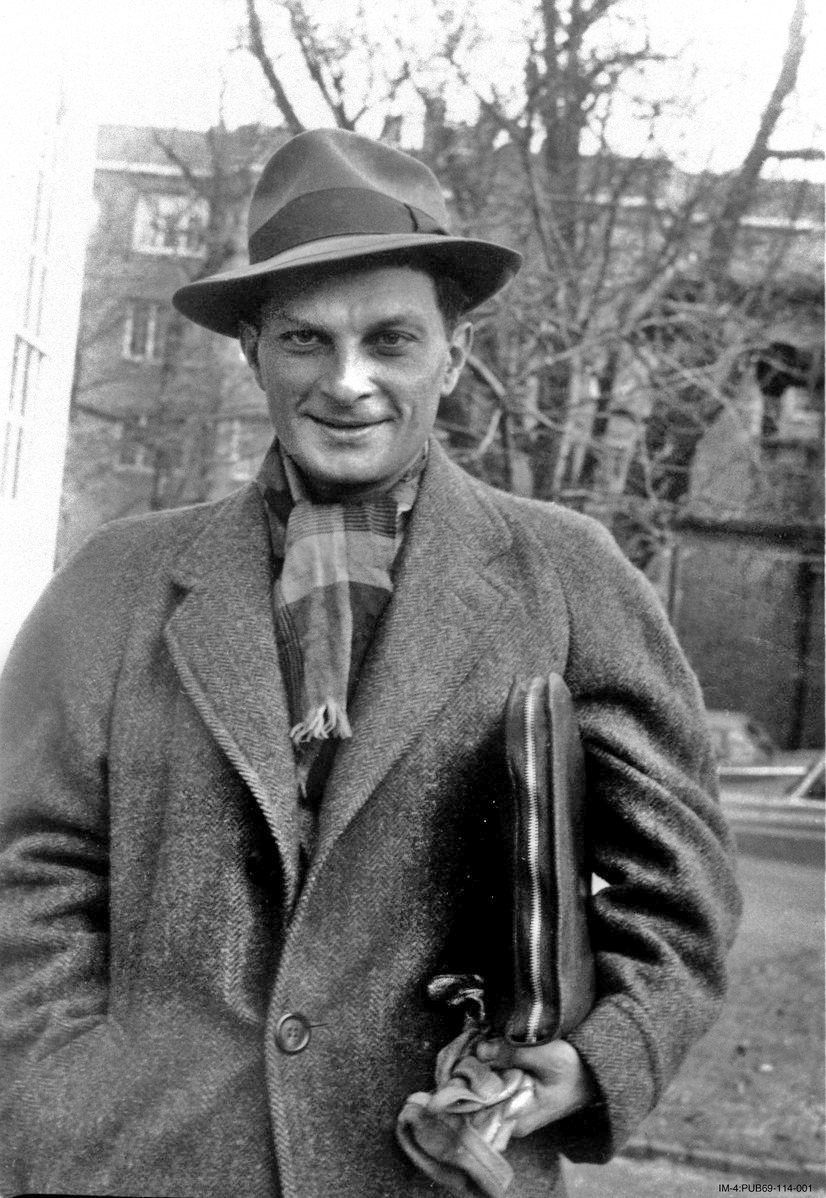
\includegraphics[height=6.0cm]{StanislawUlam.png}}
    \pause
    \subfigure[John von Newmann]{
    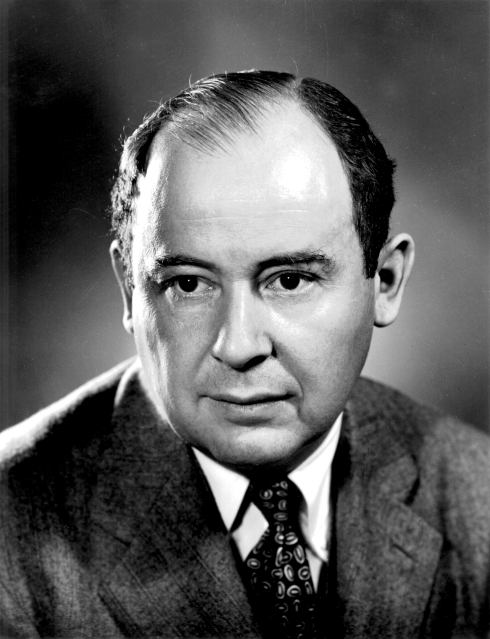
\includegraphics[height=6.0cm]{JohnvonNeumann.png}}
  \end{figure}
\end{frame}

\begin{frame}
  \frametitle{История}
  \begin{figure}[t]
    \centering
    \subfigure[Electronic Numerical Integrator And Computer]{
    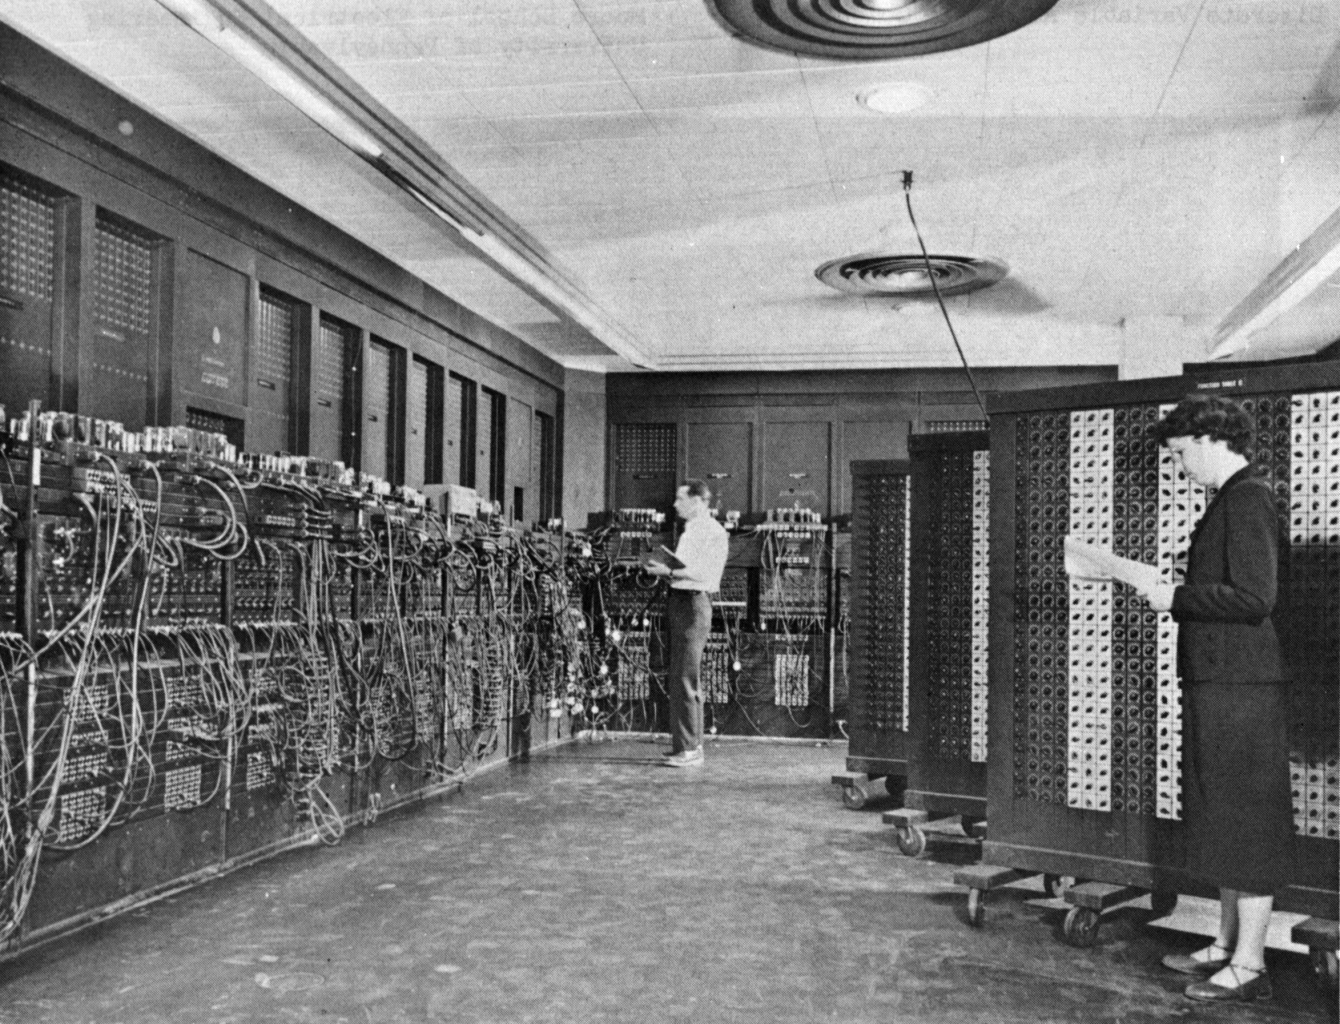
\includegraphics[height=6.5cm]{Eniac.jpg}}
  \end{figure}
\end{frame}
\begin{frame}
  \frametitle{История}
  \begin{figure}[t]
    \centering
    \subfigure[Fat Man]{
    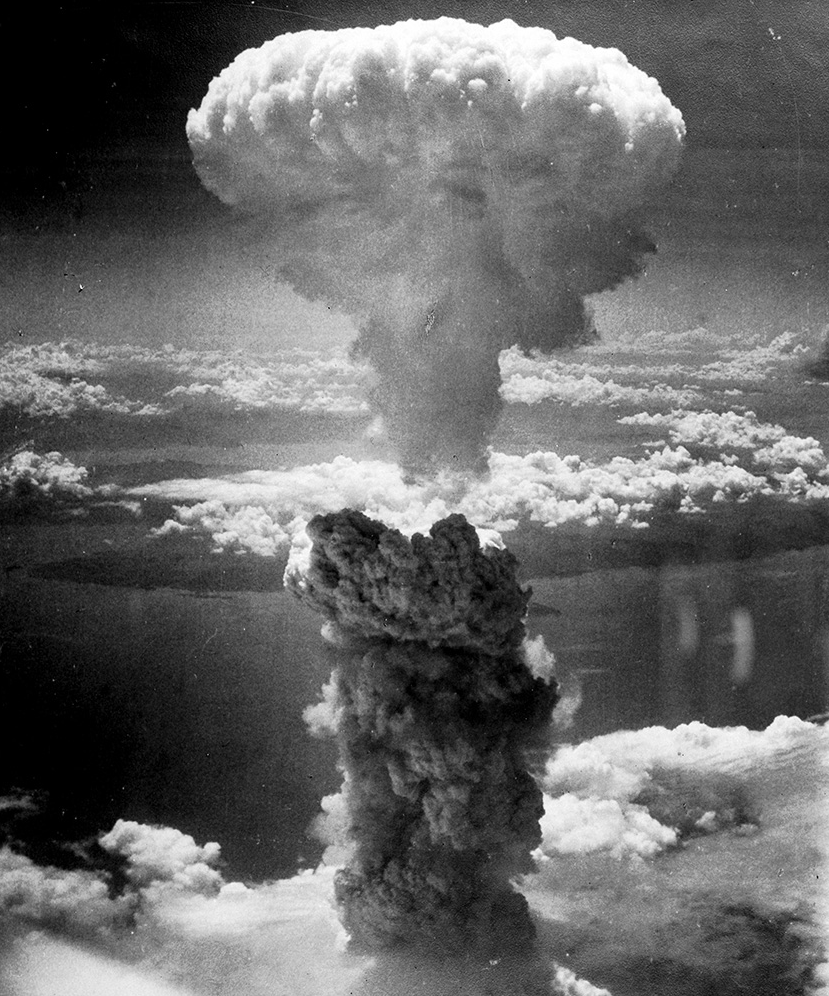
\includegraphics[height=6.5cm]{fatman.png}}
  \end{figure}
\end{frame}
